\section{Analoge Schaltung} 
\label{sec:analoge_schaltung}
Im Kapitel werden die verschiedenen analogen Schaltungsteile näher erläutert. Zuerst werden die verschiedenen Schaltungsteile auf dem Layer 1 erläutert. Dies beinhaltet die Speisung, Sicherheitsaspekte und die Messung. Danach werden die Bestandteile der Signalaufbereitung näher betrachtet.

\subsection{Layer 1}%Marc 1 Seite
%%%%%%%%%%%%%%%%%%%%%%%%%%%%%%%%%%%%%%%%%%%%%%%%%%%%%%%%%%%%%%%%%%%%%%%%%%%
Der erste Layer ist für alle Schaltungsteile mit 230V, sowie für die Verbindung nach aussen zuständig. Abbildung \ref{fig:first_layer} zeigt den groben Aufbau. Das genaue Schema befindet sich im Anhang.

\begin{figure}[H]
\begin{center}
	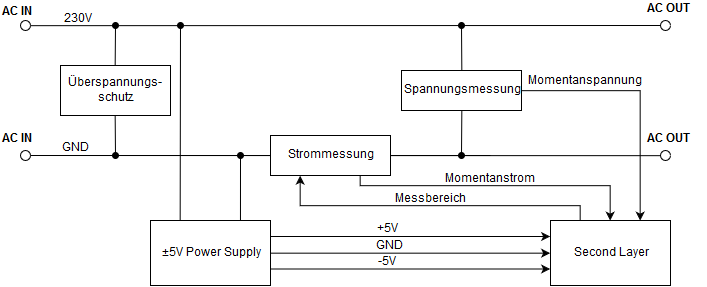
\includegraphics[width=160mm]{images/first_layer.png}
	\caption{Blockschaltbild des ersten Layers des Leistungsmessgerätes} %picture caption
	\label{fig:first_layer}
\end{center}
\end{figure}

\subsubsection*{Überspannungsschutz:}
Der Überspannungsschutz schützt das Gerät vor Spannungen über 400V. Der Rest des Gerätes ist somit für bis 400V ausgelegt. Da das Gerät mit Wechselstrom betrieben wird, ist ein Verpolungsschutz unnötig. Einzig wird die Masse des Gerätes auf 230VAC schweben, falls das Gerät verpolt betrieben wird.

\subsubsection*{Strommessung:}
Für die Strommessung stehen zwei Mess-Schunts zu Verfügung. Zum einen ein $50m\Omega$ Widerstand und zum anderen ein $1m\Omega$-Widerstand, welcher mit einem Relais parallel zum Ersten geschaltet wird. Durch die Parallelschaltung kann der Messbereich bei Betrieb umgeschaltet werden, ohne einen Unterbruch zu provozieren. Aufgrund induktiven Lasten könnten hohe Spannungen entstehen, die die Schaltung zerstören würden. Zudem kann somit eine unterbruchsfreie Versorgung der Last gewährleistet werden. Für die Messung wird die Spannung vor dem Shunt bezüglich Masse (GND) gemessen.

\subsubsection*{Spannungsmessung:}
Die Spannung wird durch einen Spannungsteiler mit dem Verhältnis $\frac{7.5}{1000}$ gemessen, was bei einer Spannung von $\pm 400V$ zu einem Messsignal von $\pm 3V$ führt. Da der Messbereich des ADCs $\pm 2.5V$ beträgt, können maximal Spannungen von $\pm 333V$ gemessen werden.

\subsubsection*{Power Supply:}
Das Netzteil versorgt den gesamten Gleichstromteil der Schaltung. Es stellt einen maximalen Strom von $400mA$ zur Verfügung.

%%%%%%%%%%%%%%%%%%%%%%%%%%%%%%%%%%%%%%%%%%%%%%%%%%%%%%%%%%%%%%%%%%%%%%%%%%%
\subsection{Filter}

Wie schon im Kapitel technische Grundlagen 3.2 erwähnt, werden die Filter benötigt um harmonische Oberwellen herauszufiltern. Gemäss Lastenheft sollen Oberwellen ab 5kHz nicht mehr im Signal sichtbar sein. Darum müssen Oberwellen die eine höhere Frequenz haben, unterdrückt werden damit diese nicht die Messung verfälschen.

\begin{figure}[H]
\begin{center}
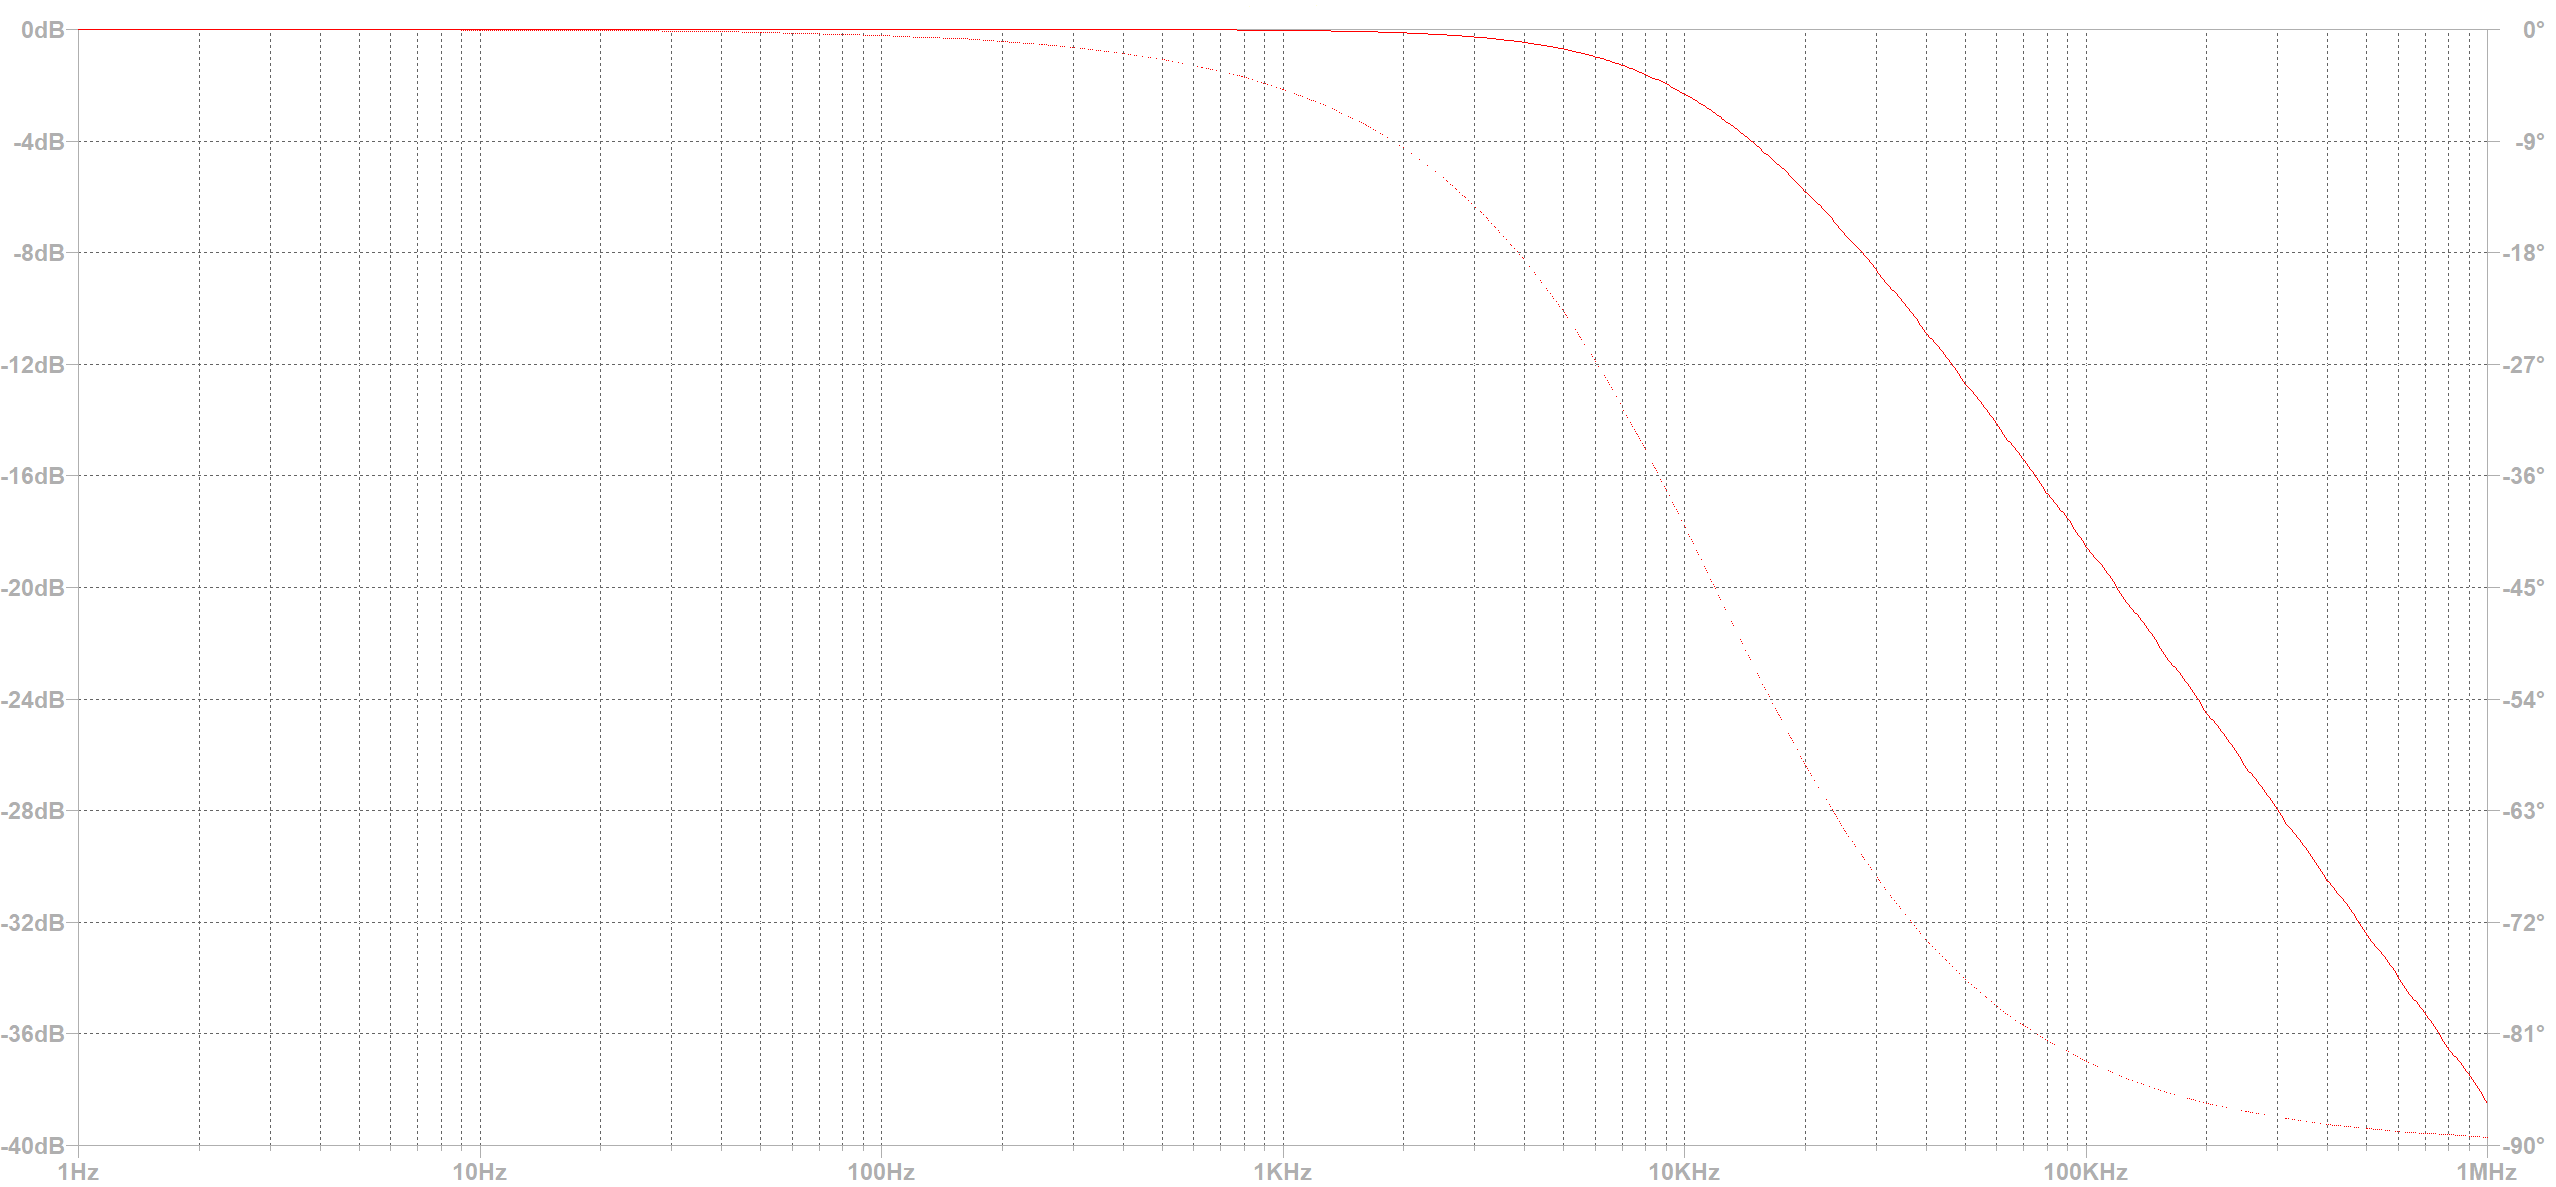
\includegraphics[width=0.9\textwidth]{images/Analoge_Schaltung_Frequenzgang.png}
\caption{Frequenzgang Tiefpass-Filter 1. Ordnung}
\end{center}
\end{figure}


Tiefpass-Filter sind geeignet, weil sie höhere Frequenzen unterdrücken und tiefe Frequenzen passieren lassen. Auf dem nebenstehenden Bild ist ein typischer Frequenzgang eines Tiefpass-Filters 1. Ordnung zu sehen. Da für das Projekt die Signale auch verstärkt werden müssen, sind aktive Filter naheliegend.\cite{ant}


\subsubsection*{Dimensionierung}

Die Wahl fiel auf Butterworth-Filter mit Sallen/Key-Topologie 2. Ordnung. Diese Topologie bietet den Vorteil, dass sie nicht invertierend ist. Dadurch ist ein Operationsverstärker ausreichend pro Signalpfad. Die Butterworth-Koeffizienten bieten den Vorteil, dass sie flach sind im Durchlassbereich und einen relativ eckigen Übergang haben.\cite{wiki}



\begin{figure}[H]
\begin{center}
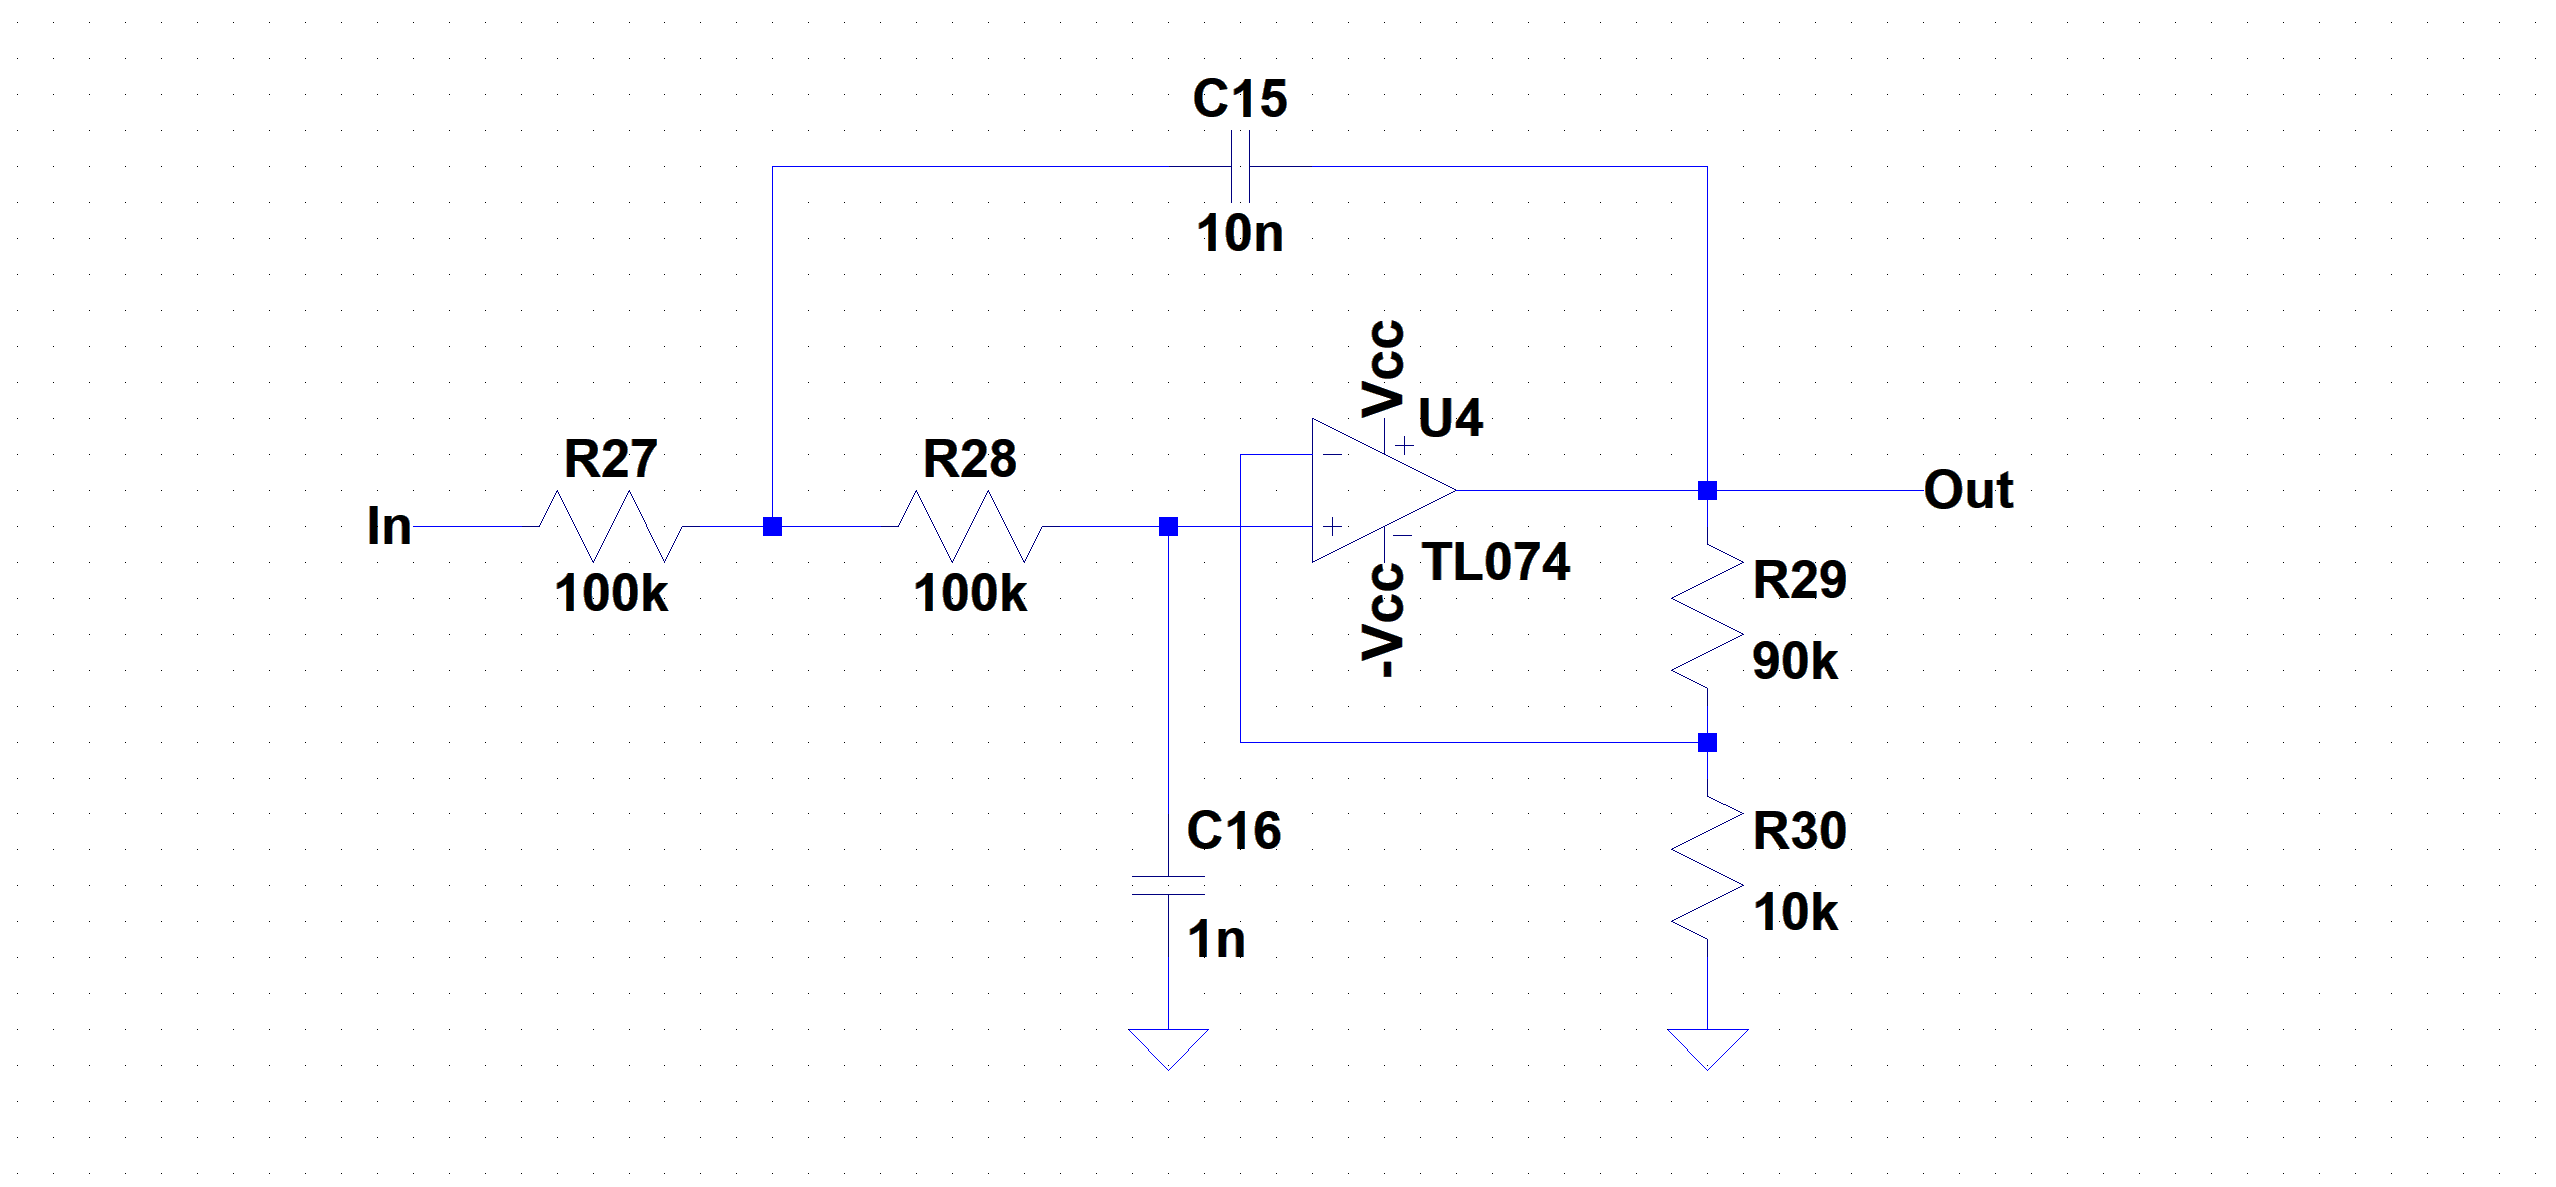
\includegraphics[width=0.9\textwidth]{images/Analoge_Schaltung_Sallen.png}
\caption{Sallen/Key-Topologie Tiefpass-Filter 2. Ordnung}
\end{center}
\end{figure}


\subsubsection*{Auswahl Operationsverstärker}
An den Operationsverstärker wurden praktisch keine Anforderungen gestellt. Er soll ein GWP\cite{wiki} von mindestens 800kHz besitzen und nicht Rail-to-Rail sein. Ausserdem werden vier Operationsverstärker benötigt. Dies ist der \textbf{TL074}, der praktischerweise 4 Operationsverstärker in einem Gehäuse vereint. Die passiven Bauteile wurden mithilfe einer Formel\cite{fail} aus dem Internet erstellt, die sich im Laufe des Projektes als falsch herausstellte.

\subsubsection*{Falsche Filter}
Nachdem der Print gefertigt war, wurde beim Testen festgestellt, dass die Filter instabil laufen. Es wurde überlesen, dass mit der Sallen/Key-Filtertopologie nur Verstärkungen bis drei realisierbar sind. Bei höheren Verstärkungen können diese instabil werden. Diesen schwerwiegenden Fehler wurde gemacht. Aus der Not wurden die Filter umgebaut in einen passiven Filter 1. Ordnung, gefolgt von einer Verstärkerschaltung. Dafür musste nur der Kondensator C15 entlötet werden, damit ein Unterbruch entsteht, und für den R27 wurde eine Drahtbrücke eingelötet.

\begin{figure}[H]
\begin{center}
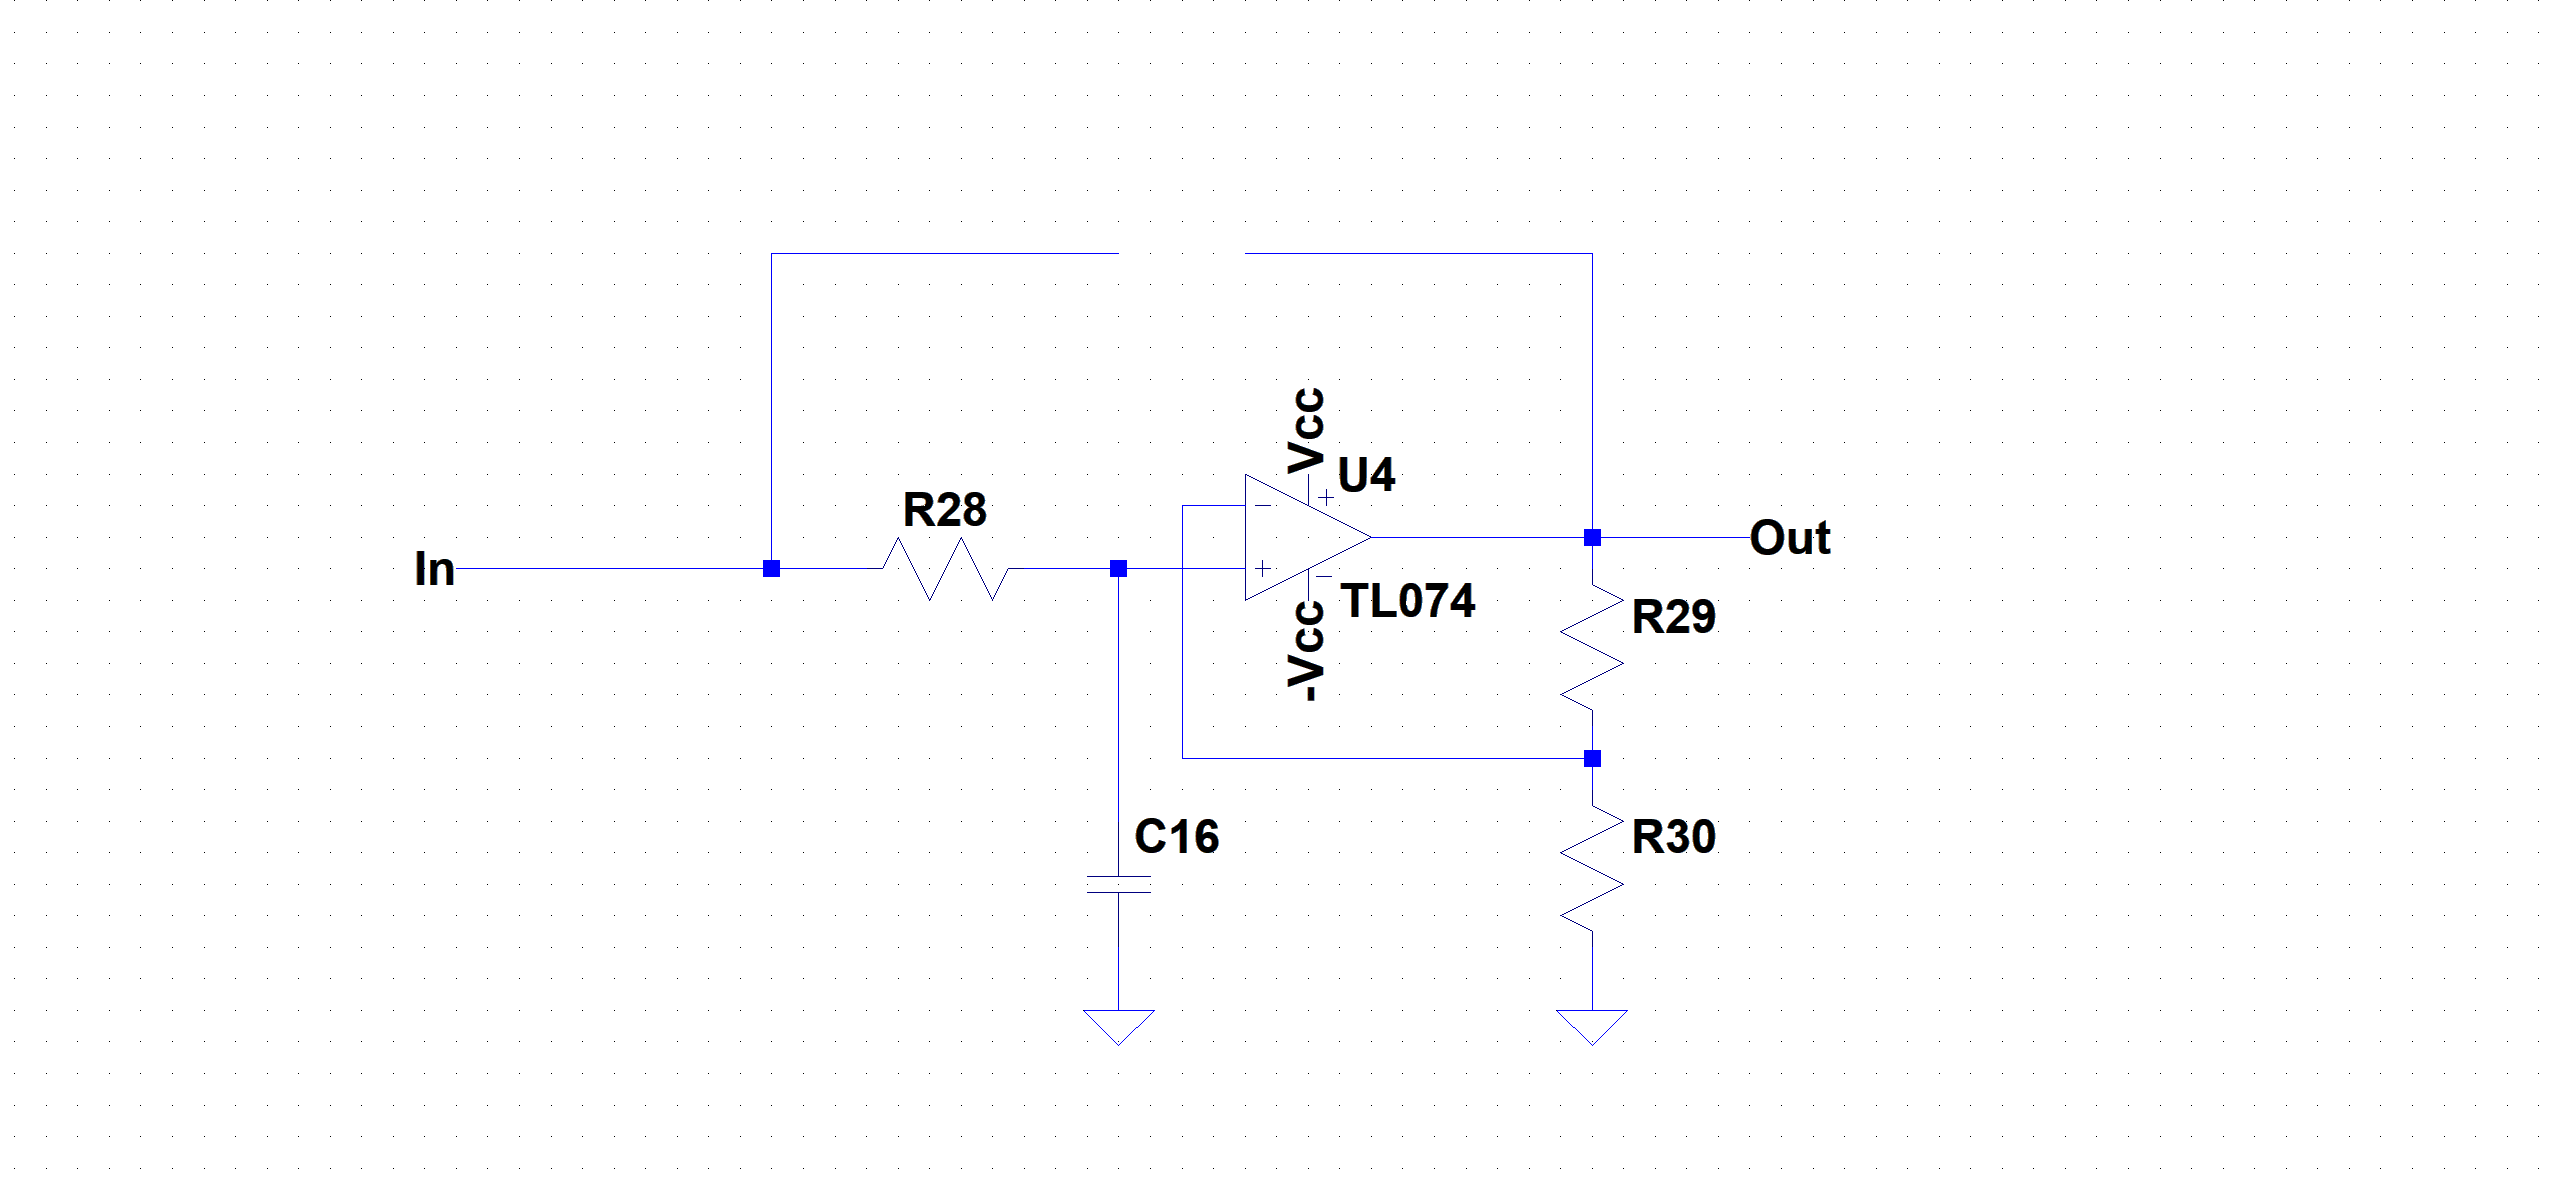
\includegraphics[width=0.9\textwidth]{images/Analoge_Schaltung_Sallentopassive.png}
\caption{Umgebautes Sallen/Key zu passivem Filter 1. Ordnung}
\end{center}
\end{figure}

Die Dimensionierung der neuen Schaltung ist mithilfe der nachfolgenden Formeln geschehen. Die Verstärkungen konnten beibehalten werden. Die passiven Filter mussten neu berechnet werden.\cite{wiki}

\begin{equation}
f_g=\frac{1}{2 \cdot \pi \cdot R_{28} \cdot C_{16}}
\label{eq:Grenzfrequenz}
\end{equation}

\begin{equation}
A=1+\frac{R_{29}}{R_{30}}
\label{eq:Verstärkung}
\end{equation}

%%%%%%%%%%%%%%%%%%%%%%%%%%%%%%%%%%%%%%%%%%%%%%%%%%%%%%%%%%%%%%%%%%%%%%%%%%%
\subsection{Einkoppelung}
Das Signal nach der Filterung und der Verstärkung beträgt $\pm 2.5V$. Um dieses Signal anzuheben auf eine für den Mikrocontroller angepasste Grösse, wird eine DC-Spannung eingekoppelt. Nach der Einkoppelung von $2.5V$ bewegt sich das Signal innerhalb von $0V$ bis $5V$. Dies wurde mit folgender Schaltung realisiert, siehe Abbildung \ref{fig:Einkoppelung}.


\begin{figure}[H]
\begin{center}
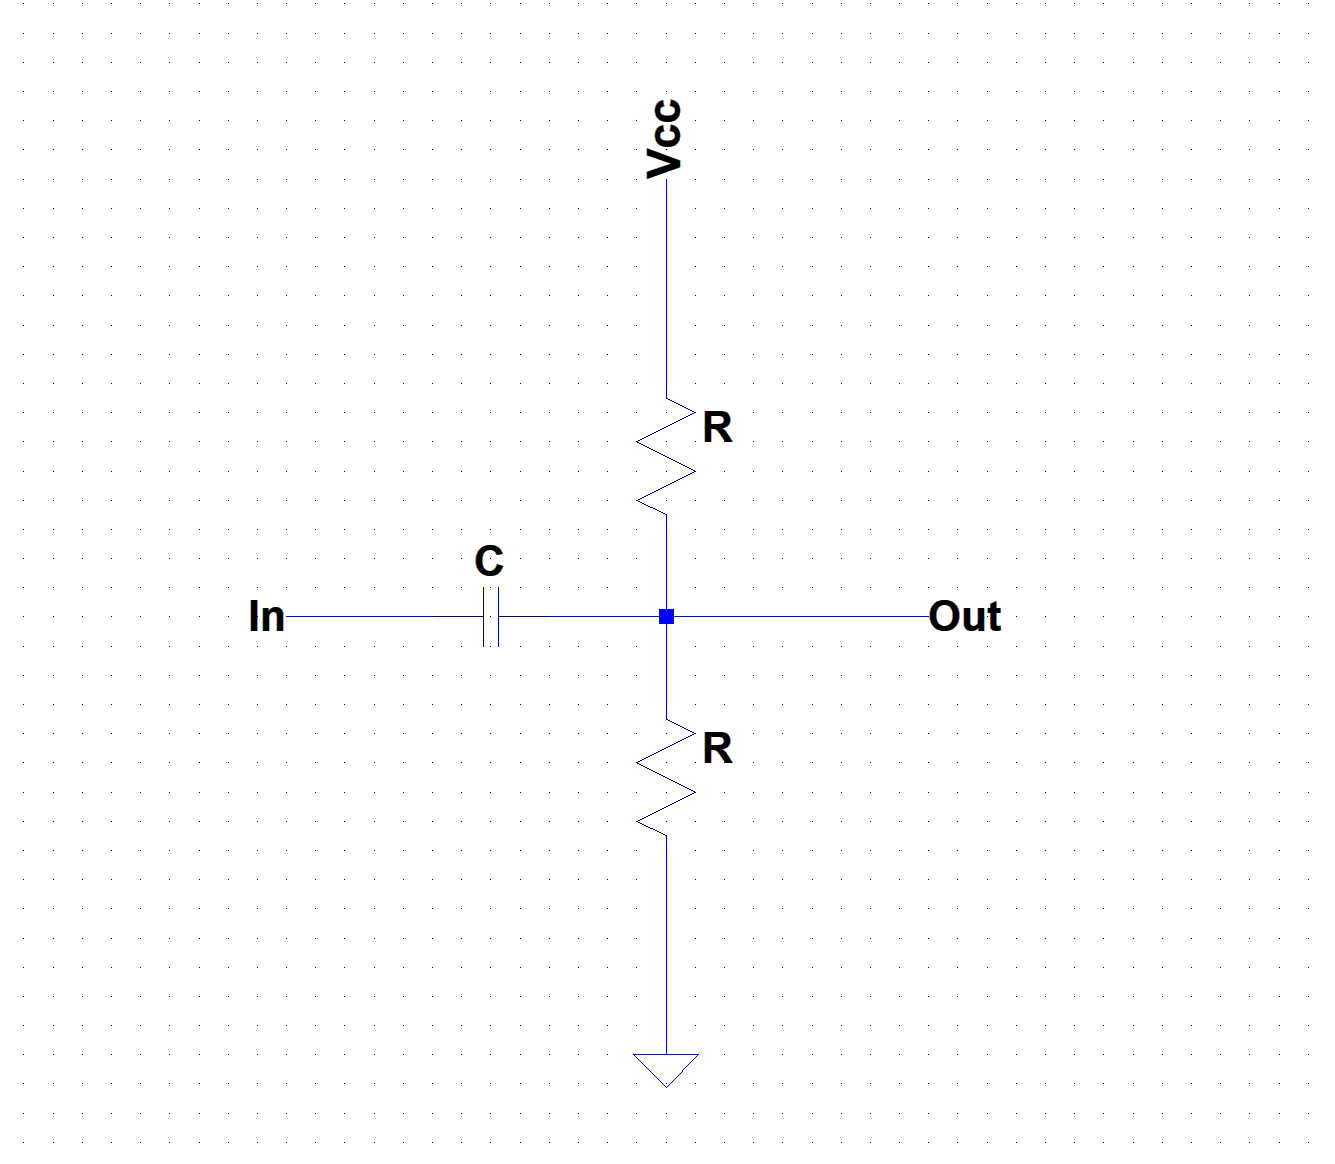
\includegraphics[width=0.9\textwidth]{images/Analoge_Schaltung_Einkoppelung.png}
\caption{Einkoppelung}
\label{fig:Einkoppelung}
\end{center}
\end{figure}

Um diese Schaltung zu dimensionieren, muss eine AC- und eine DC-Betrachtung gemacht werden.


Für die AC-Betrachtung ist sie ein Hochpassfilter 1. Ordnung. Dieses Hochpassfilter soll alle Frequenzen passieren lassen ausser Gleichstrom. Für die Dimensionierung kann dieselbe Formel \eqref{eq:Grenzfrequenz} wie für die Tiefpass-Filter verwendet werden. Jedoch wird die Grenzfrequenz $f_g$ auf $0.5 Hz$ gesetzt. $R_{28}$ setzt sich aus den  zwei parallel gesetzten Widerständen zusammen.


Für die DC-Betrachtung entspricht die Schaltung einem Spannungsteiler. Der Kondensator stellt in dieser Betrachtung einen Unterbruch dar. Die Widerstände sollten gross gewählt werden, damit die Verluste klein bleiben. Gleichzeitig muss mit den Anforderungen des Hochpassfilters einen Kompromiss gefunden werden. Für unser Projekt war schlussendlich die Grösse des Kondensators ausschlaggebend. Je grösser der Kondensator ist desto kleiner wird die Verlustleistung. Der grösste Kondensator der als SMD\cite{wikiSMD} erhältlich ist wurde verwendet.

%%%%%%%%%%%%%%%%%%%%%%%%%%%%%%%%%%%%%%%%%%%%%%%%%%%%%%%%%%%%%%%%%%%%%%%%%%%
\subsection{Sicherheitsschaltung}

Um die Eingänge des Mikrocontroller zu schützen, wurde eine Sicherheitsschaltung realisiert. Diese schützt den Eingang vor Überspannungen und Unterspannungen. Die obere Diode schaltet, sobald das Eingangssignal oberhalb von Vcc plus der Forward-Voltage der Diode ist. In diesem Fall entsteht ein Kurzschluss zwischen GND und Vcc durch den Operationsverstärker. Um den Strom zu begrenzen, ist der Widerstand vorhanden. Gleichzeitig bildet der Widerstand mit dem Kondensator zusammen ein weiteres Tiefpass-Filter, das hochfrequente Störungen abhalten soll.  Die Grenzfrequenz dieses Filters muss höher sein, als die Grenzfrequenz des ersten Filters, damit es nicht das Signal verfälscht.


\begin{figure}[H]
\begin{center}
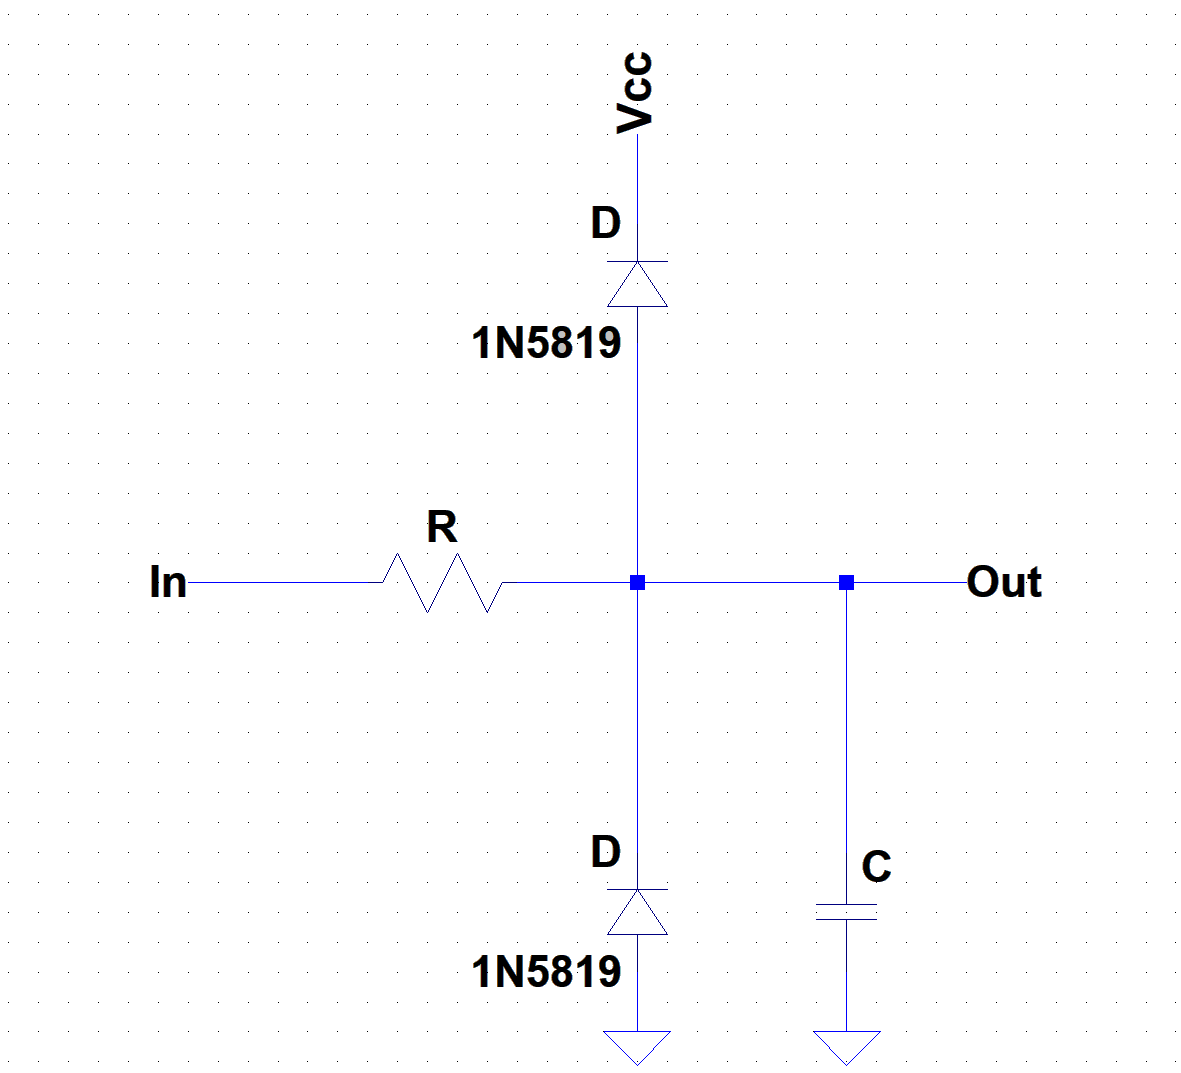
\includegraphics[width=0.9\textwidth]{images/Analoge_Schaltung_Sicherung.png}
\caption{Sicherheitsschaltung}
\label{fig:Sicherheitsschaltung}
\end{center}
\end{figure}

\subsection{Genauigkeit}%Marc 1 Seite
%%%%%%%%%%%%%%%%%%%%%%%%%%%%%%%%%%%%%%%%%%%%%%%%%%%%%%%%%%%%%%%%%%%%%%%%%%%
Die Genauigkeit im analogen Schaltungsteil hängt zum einen von den Toleranzen und Ungenauigkeiten der verwendeten Bauteile und zum anderen von der Auflösung des ADCs ab, welcher die Grenze zwischen analog und digital bildet. Abbildung \ref{fig:genauigkeit} zeigt den Messpfad mit den möglichen Teilen, in welchen Ungenauigkeiten entstehen können und werden.

\begin{figure}[htb]
	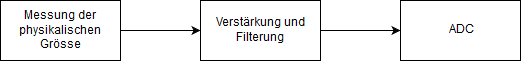
\includegraphics[width=160mm]{images/Analoge_Schaltung_genauigkeit.png}
	\caption{Messpfad} %picture caption  
	\label{fig:genauigkeit}
\end{figure}

Nachfolgend werden die möglichen Fehler der einzelnen Blöcke in Abbildung \ref{fig:genauigkeit} erläutert.

\subsubsection*{Messung der physikalischen Grösse}
Der Strom und die Spannung werden jeweils als Spannung über einen bestimmten Widerstand gemessen.Wie aus dem Schema im Anhang ersichtlich, lässt sich der Strom über das Ohmsche Gesetz berechnen und die Spannung über einen Spannungsteiler. 

\begin{equation}
I = \frac{U_{mess}}{R_{mess}} \to I = \frac{U_{mess}}{R_{mess} + R_{toleranz}} = \frac{U_{mess}}{R_{mess}} \cdot \frac{1}{a}
\end{equation}

\[a = \frac{R_{mess} + R_{toleranz}}{R_{mess}}\]

\begin{equation}
U = U_{mess} \cdot \frac{R_{tot}}{R_{mess}} \to U = U_{mess} \cdot \frac{R_{tot} + R_{toleranz1,2}}{R_{mess}+R_{toleranz2}} = U_{mess} \cdot \frac{R_{tot}}{R_{mess}} \cdot \frac{1}{b}
\end{equation}

\[b = \frac{\frac{R_{tot} + R_{toleranz1,2}}{R_{tot}}}{\frac{R_{tot} + R_{toleranz2}}{R_{tot}}}\]

Somit ergeben die Toleranzen der Widerstände konstante faktorielle Fehler $a$ und $b$, welche durch eine Multiplikation während der digitalen Weiterverarbeitung des Messsignals behoben werden können.





\subsubsection*{Verstärkung, Einkopplung und Filterung}
Der Strom und die Spannung werden im jeweiligen Kanal verstärkt, um 2.5V angehoben und gefiltert. Da die Filterung erst ab 10kHz abschneidet, sind die Fehler im Durchlassbereich vernachlässigbar. Die Verstärkung wird durch einen nicht invertierenden Operationsverstärker erreicht.

\begin{equation}
U_{out} = U_{in} \left( 1+\frac{R_2}{R_1} \right) \to U_{out} = U_{in} \left( 1+\frac{R_2+R_{toleranz1}}{R_1+R_{toleranz2}} \right) = U_{in}\left(1+\frac{R_2}{R_1}\right) \cdot \frac{1}{a}
\end{equation}

Somit kann der Fehler wie im vorherigen Abschnitt durch eine Multiplikation mit einer Konstante kompensiert werden.

Bei der Einkopplung wird die Spannung an einem Spannungsteiler zum Signal hinzuaddiert (siehe Schema im Anhang).

\begin{equation}
U_{out} = U_{in} + \frac{V_{CC} \cdot R_2}{R_1+R_2} \to U_{out} = U_{in} + \frac{V_{CC} \cdot (R_2 + R_{toleranz2})}{R_1+R_2 + R_{toleranz1,2}} =  U_{in} + \frac{V_{CC} \cdot R_2}{R_1+R_2} + b
\end{equation}

Daher wird bei diesem Fehler im Gegensatz zu den anderen eine zusätzliche Konstante dazu addiert, um den durch die Widerstandstoleranzen entstandenen Fehler zu entfernen.
 
\subsubsection*{Analog-Digital-Wandler}
Bei der Konvertierung eines analogen Signals zu einem Digitalem gibt es zwingendermassen einen Informationsverlust durch die Quantisierung des Signals. Da für dieses Gerät ein 10 Bit ADC verwendet wird, hat das digitale Signal eine Auflösung von 1024 Werten. Für die vier Messkanäle ergeben sich folgende Toleranzen in der Tabelle \ref{tab:auflösung}.


\begin{table}[H]
\centering
\begin{tabular}{|l|l|l|l|l|}
\hline
Messung     & Spannung  & \multicolumn{3}{c|}{Strom}     \\ \hline
Messbereich & $\pm333V$ & $\pm15A$ & $\pm5A$ & $\pm0.5A$ \\ \hline
Auflösung   & $0.65V$   & $29mA$   & $9.8mA$ & $0.98mA$  \\ \hline
\end{tabular}
\caption{Auflösung der Messbereiche}
\label{tab:auflösung}
\end{table}

\subsubsection*{Resultierende Genauigkeit} 
Die Ungenauigkeit setzt sich zum einen durch den Informationsverlust der Quantisierung am ADC zusammen. Zum Anderen werden zusätzliche Ungenauigkeiten durch elektromagnetische Einkopplungen der umgebenden Schaltung und nicht einberechnete Faktoren der Schaltung wie zum Beispiel Leitungswiderstände entstehen. Die Fehler, welche durch die Toleranzen der Bauteile entstehen, können wie in den vorherigen Abschnitten beschrieben durch Multiplikationen und Additionen kompensiert werden.



\pagebreak